\chapter{Inertia}\label{app:Inertia}
One set of parameters in the model is the inertia of the quadcopter around its axes, roll, pitch and yaw. There are different approaches to find the inertia, but to get a good starting point the quadcopter is split op in several masses and the inertia is found analytically.

The quadcopter is first decomposed into a set of objects for which the inertia is well defined, this is done in \autoref{fig:quadcopterMasses}.

\begin{figure}[H]
  \centering
  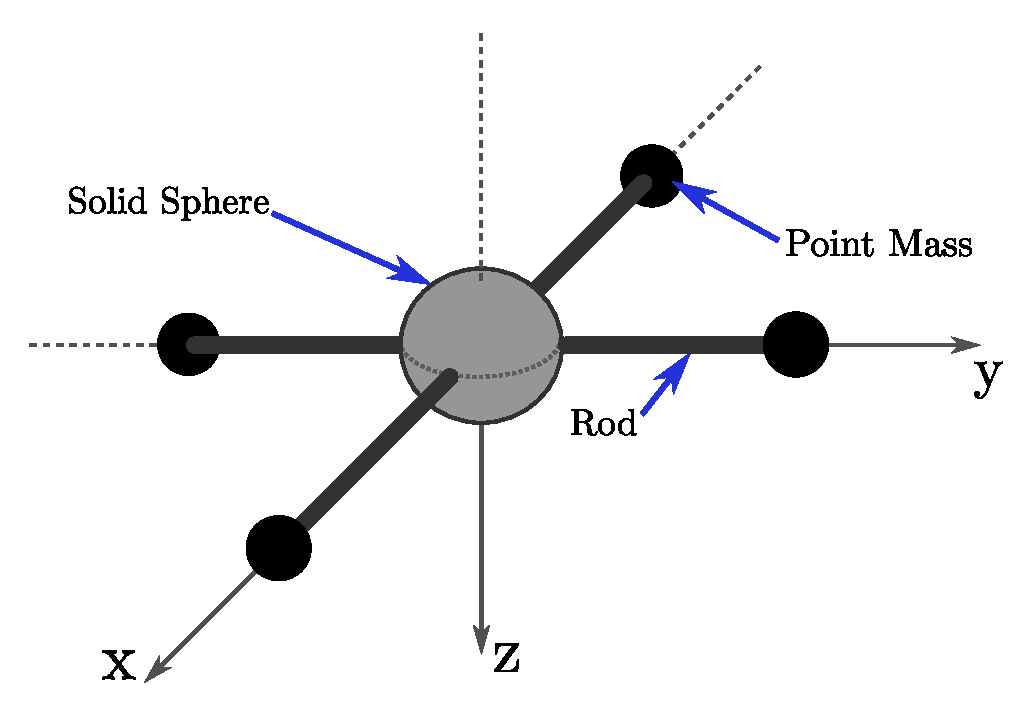
\includegraphics[width=.6\linewidth]{figures/quadcopterMasses}
  \caption{Decomposition of the quadcopter into objects for which the inertia is well defined.}
  \label{fig:quadcopterMasses}
\end{figure}

The inertia must be calculated around axes for which the roll, pitch and yaw angles are defined, that is, the x-, y- and z-axis. Since the quadcopter is controlled in plus configuration, the x- and y-axis aligns with the four arms, as seen in \autoref{fig:quadcopterMasses}.

The objects are analyzed individually around the center of mass, CM, see \autoref{fig:inertiaObjects}, after which the inertias are summed for each axis of rotation.

\begin{figure}[H]
  \centering
  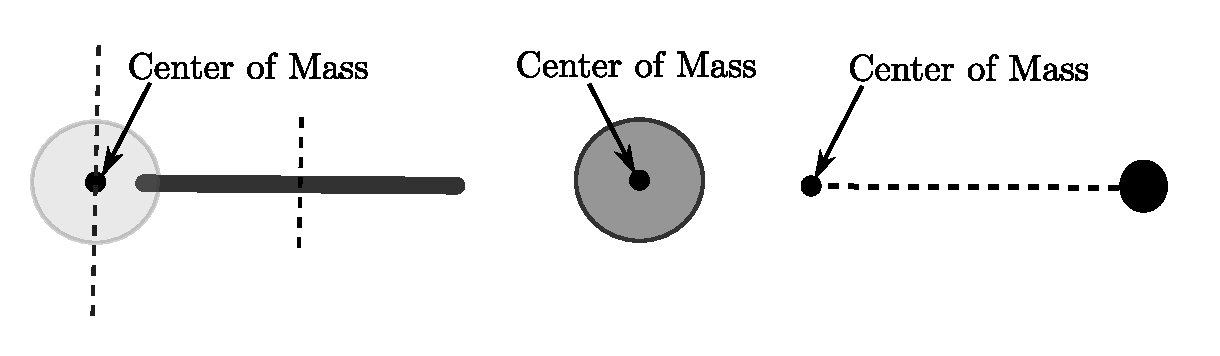
\includegraphics[width=.9\linewidth]{figures/inertiaObjects}
  \caption{The masses with respect to the center of mass of the quadcopter and axes of rotation.}
  \label{fig:inertiaObjects}
\end{figure}

To calculate the inertias it is necessary to distribute the mass of the quadcopter between the decomposed objects in \autoref{fig:quadcopterMasses}. To do this the motors and propellers are weighed and considered to be the point mass, the arm and ESC are weighed and considered to be the rod. Finally the entire quadcopter was weighed and the weight of the other objects subtracted to find the mass of the sphere.\\

The inertia of the sphere is directly given by
\begin{flalign}
  I_s &= \frac{2}{5}  m_s r_s^2    \unit{kg \cdot m ^2}
\end{flalign}
%
\begin{where}
  \va{I_s}  {is the moment of inertia around the CM of the quadcopter}  {kg \cdot m ^2}
  \va{m_s}  {is the mass of the sphere}  {kg}
  \va{r_s}  {is the radius of the sphere}  {m}
\end{where}

For a point mass the moment of inertia around the CM of the quadcopter is given by
\begin{flalign}
  I_p &= m_p d_p ^2   \unit{kg \cdot m ^2}
\end{flalign}
%
\begin{where}
  \va{I_p}  {is the moment of inertia around the CM of the quadcopter}  {kg \cdot m ^2}
  \va{m_p}  {is the mass of the point}  {kg}
  \va{d_p}  {is the distance from the point mass to the CM of the quadcopter}  {m}
\end{where}

To calculate the moment of inertia of the rod, it is first evaluated around its own center of mass, see \autoref{fig:inertiaObjects}. Then by use of the parallel axis theorem the inertia is moved, such that it is described around the center of mass of the quadcopter.

The parallel axis theorem states that any mass with known inertia around an axis can be described around a parallel axis by adding its mass multiplied by the distance between the parallel axes squared.\\

\pagebreak
For the rod this yields the following,
\begin{flalign}
  I_r &= \frac{1}{12}  m_r L_r ^2  + m_r d_r^2  \unit{kg \cdot m ^2}
\end{flalign}
%
\begin{where}
  \va{I_r} {is the moment of inertia around CM of the rod}  {kg \cdot m ^2}
  \va{m_r} {is the mass of the rod}  {kg}
  \va{L_r}   {is the length of the rod}  {m}
  \va{d_r}   {is the distance from CM of the rod to the CM of the quadcopter}{m}
\end{where}

The found inertias are summed for each axis of rotation to obtain the final inertias of the quadcopter.
\begin{flalign}
  I_x &=  I_s + 2 I_p + 2 I_r    \unit{kg \cdot m ^2}\\
  I_y &=  I_s + 2 I_p + 2 I_r    \unit{kg \cdot m ^2}\\
  I_z &=  I_s + 4 I_p + 4 I r    \unit{kg \cdot m ^2}
\end{flalign}
%
\begin{where}
  \va{I_x} {is the moment of inertia around the x-axis}  {kg \cdot m ^2}
  \va{I_y} {is the moment of inertia around the y-axis}  {kg \cdot m ^2}
  \va{I_z} {is the moment of inertia around the z-axis}  {kg \cdot m ^2}
\end{where}

In \autoref{tab:quadcopterMasses} the measured quantities are given.

\begin{table}[H]
  \centering
  \begin{tabular}{|l|l|l|l|l|l|l|}
    \hline%----------------------------------------------------------------------------------------------------------
    $m_s$        & $m_p$          & $m_r$          & $r_s$         & $d_p$         & $L_r$         & $d_r$         \\
    \hline%----------------------------------------------------------------------------------------------------------
    \SI{0.4}{kg} & \SI{0.074}{kg} & \SI{0.075}{kg} & \SI{0.065}{m} & \SI{0.120}{m} & \SI{0.165}{m} & \SI{0.225}{m} \\
    \hline%----------------------------------------------------------------------------------------------------------
  \end{tabular}
  \caption{Measured masses on of the quadcopter.}
  \label{tab:quadcopterMasses}
\end{table}

Inserting the measured quantities in the formulas yields the following,
\begin{flalign}
  I_s &= \frac{2}{5}  0.4 \times 0.065^2                             &= 0.6760 &\times 10^{-3}  &\ \si{kg \cdot m ^2} &\hspace{1cm}& \\
  I_p &= 0.074 \times 0.120^2                                        &= 0.0011 & &\ \si{kg \cdot m ^2} &\hspace{2cm}& \\
  I_r &= \frac{1}{12}  0.075 \times 0.165 ^2  + 0.075 \times 0.225^2 &= 0.0040 & &\ \si{kg \cdot m ^2} &\hspace{2cm}& \\
  I_x &= 0.6760 + 2 \times 0.0011 + 2 \times 0.0040                  &= 0.0107 & &\ \si{kg \cdot m ^2} &\hspace{2cm}& \\
  I_y &= 0.6760 + 2 \times 0.0011 + 2 \times 0.0040                  &= 0.0107 & &\ \si{kg \cdot m ^2} &\hspace{2cm}& \\
  I_z &= 0.6760 + 4 \times 0.0011 + 4 \times 0.0040                  &= 0.0208 & &\ \si{kg \cdot m ^2} &\hspace{2cm}&
\end{flalign}